\chapter{Convolutional Neural Network}\label{ch:cnn}
Le \textbf{Convolutional Neural Network} (CNN) sono reti neurali pensate per elaborare immagini e, più in generale, dati organizzati su una griglia. In questo capitolo partiamo dai limiti di un MLP quando l'input è un'immagine, introduciamo l'operazione di convoluzione e vediamo come i suoi parametri (padding, stride e dilation) determinano la forma dell'output. Infine vediamo gli altri layer che compongono una CNN (attivazioni, normalizzazione, pooling e fully connected) e alcune regole pratiche per progettarla.

\section{Dalle reti neurali alle immagini}
\subsection{Representation learning}
Riprendiamo un MLP con un solo hidden layer, ad esempio con 4 input e 3 output. Rispetto al capitolo~\ref{ch:ripasso}, qui scriviamo il bias $b$ separato dai pesi $\vartheta$, come nelle slide del corso. La rete calcola:
\[
F_\vartheta(x) = \vartheta_2\, f(\vartheta_1 x + b_1) + b_2
\]
ed esegue quindi due trasformazioni:
\begin{enumerate}
    \item trasforma l'input $x$ in $a(x) = f(\vartheta_1 x + b_1)$.
    \item trasforma il risultato intermedio $a(x)$ nell'output $h(x) = \vartheta_2\, a(x) + b_2$.
\end{enumerate}
Il risultato intermedio $a(x)$ è una \textbf{rappresentazione} di $x$, e non è scelto da noi ma appreso: l'MLP sta facendo \textbf{representation learning}\footnote{Il termine \textit{representation learning} si riferisce alla capacità di una rete neurale di apprendere automaticamente rappresentazioni utili dei dati di input.}.

In generale, una rete neurale implementa una funzione che mappa l'input $x$ nell'output $y$, dati i parametri $\vartheta$:
\[
y = h(x; \vartheta) = F_\vartheta(x).
\]
Se abbiamo un numero sufficiente di coppie $\langle x^{(i)}, y^{(i)}\rangle$ (il dataset), possiamo cercare i parametri $\vartheta$ ottimali, ovvero quelli per cui
\[
\sum_i \mathrm{loss}\big(y^{(i)}, h(x^{(i)}; \vartheta)\big)
\]
è minima, dove la funzione di loss misura l'errore commesso da $h$ nel predire $y$. La ricerca dei parametri ottimali è la procedura di \textbf{training}, e l'algoritmo più usato è la backpropagation vista nel capitolo~\ref{ch:backprop}: poiché $h$ è derivabile rispetto a $\vartheta$, funziona secondo il principio della discesa del gradiente.

\paragraph{Esempio: regressione.}
Vogliamo predire il consumo di un'automobile, in miglia per gallone (mpg), a partire da tre feature: il numero di cilindri $c$, la potenza $p$ e il peso $w$. È ragionevole pensare che esista una funzione $h$ tale che
\[
\mathrm{mpg} = h(c, p, w).
\]
Come la definiamo matematicamente? Non lo facciamo: la impariamo dai dati. Il dataset \emph{Auto MPG} contiene 398 auto, e possiamo usarlo per apprendere i pesi della rete a sinistra in figura~\ref{fig:reg-class}. Trattandosi di regressione, come funzione di loss si usa la MSE.

\paragraph{Esempio: classificazione.}
Il dataset \emph{Iris} contiene 150 fiori, descritti da 4 misure e divisi in 3 specie. Vogliamo classificare un fiore a partire dalle sue misure: gli input sono quindi 4, ma quanti sono gli output? Una tecnica comune è far calcolare alla rete \textbf{un punteggio per classe} e scegliere la classe con il punteggio più alto, per cui gli output sono 3 (figura~\ref{fig:reg-class}, a destra).

In fase di training cerchiamo i pesi che assegnano un punteggio alto alla classe corretta e basso a tutte le altre. In fase di test, invece, facciamo passare il campione nella rete e scegliamo la classe con il punteggio massimo. Come loss si usa la cross-entropy, dopo aver trasformato i punteggi in probabilità con il softmax.

\begin{figure}[htbp]
\centering
\begin{tikzpicture}[>=Stealth, font=\scriptsize,
  neuron/.style={draw, circle, minimum size=5mm, inner sep=0pt},
  hid/.style={neuron, draw=Accent, fill=Accent!25}]
  % regressione
  \foreach \k/\lab in {1/cilindri, 2/potenza, 3/peso} {
    \node[neuron] (r\k) at (0,1.2-0.8*\k+0.4) {};
    \node[left] at (r\k.west) {\lab};
  }
  \foreach \k in {1,...,4} \node[hid] (rh\k) at (1.5,1.6-0.8*\k+0.4) {};
  \node[neuron] (ro) at (3,0) {};
  \node[right] at (ro.east) {mpg};
  \foreach \i in {1,2,3} \foreach \h in {1,...,4} \draw[TextGray] (r\i) -- (rh\h);
  \foreach \h in {1,...,4} \draw[TextGray] (rh\h) -- (ro);
  \node[Accent] at (1.5,1.75) {rappresentazione appresa};
  % classificazione
  \begin{scope}[xshift=7cm]
    \foreach \k in {1,...,4} \node[neuron] (c\k) at (0,1.6-0.8*\k+0.4) {};
    \draw[decorate, decoration={brace, amplitude=4pt, mirror}] (-0.35,1.3) -- (-0.35,-1.3) node[midway, left=4pt, align=right] {4 misure};
    \foreach \k in {1,...,5} \node[hid] (ch\k) at (1.5,2.0-0.8*\k+0.4) {};
    \foreach \k in {1,2,3} \node[neuron] (co\k) at (3,1.2-0.8*\k+0.4) {};
    \draw[decorate, decoration={brace, amplitude=4pt}] (3.35,1.0) -- (3.35,-1.0) node[midway, right=4pt, align=left] {3 classi};
    \foreach \i in {1,...,4} \foreach \h in {1,...,5} \draw[TextGray] (c\i) -- (ch\h);
    \foreach \h in {1,...,5} \foreach \o in {1,2,3} \draw[TextGray] (ch\h) -- (co\o);
    \node[Accent] at (1.5,2.15) {rappresentazione appresa};
  \end{scope}
\end{tikzpicture}
\caption{Due reti con un hidden layer. A sinistra, la regressione del consumo (mpg) a partire da cilindri, potenza e peso. A destra, la classificazione dei fiori del dataset Iris a partire da 4 misure, con un punteggio per ciascuna delle 3 classi. In entrambi i casi l'hidden layer (in verde petrolio) contiene la rappresentazione appresa dell'input.}
\label{fig:reg-class}
\end{figure}

\paragraph{Da shallow a deep.}
Possiamo aggiungere tutti gli hidden layer che vogliamo. Con due hidden layer, ad esempio, la rete diventa:
\[
h(x, \vartheta) = \vartheta_h\, f_2\big(\vartheta_{f_2} f_1(\vartheta_{f_1}x + b_{f_1}) + b_{f_2}\big) + b_h
\]
dove $f_1$ e $f_2$ sono le funzioni di attivazione dei due layer. Ogni layer costruisce la propria rappresentazione a partire da quella del layer precedente, per cui la rete impara delle \textbf{rappresentazioni gerarchiche}.

Serve davvero andare in profondità? In teoria no: il teorema di approssimazione universale (teorema~\ref{teo:uat}) dice che un solo hidden layer, con un numero finito di neuroni, basta ad approssimare qualunque funzione continua su un compatto di $\mathbb{R}^n$. In pratica, però, il numero di neuroni necessari può diventare enorme, ed è più utile ``scomporre'' la rete introducendo altri hidden layer.

\subsection{MLP e immagini}
Gli MLP non sono molto adatti a elaborare immagini, per tre motivi:
\begin{itemize}
    \item \textbf{Le immagini sono grandi}: anche una piccola immagine in scala di grigi di $100 \times 100$ pixel contiene 10000 valori.
    \item \textbf{Le immagini sono complesse}, e per elaborarle possono servire molti layer.
    \item Quando il numero di layer e il numero di input crescono, \textbf{il numero di parametri cresce di conseguenza}.
\end{itemize}
L'idea è quindi di ridurre il numero di parametri in ogni layer, così da poter costruire modelli più profondi.

Forniamo il seguente esempio, su cui torneremo più volte nel capitolo: il dataset \textbf{MNIST} (figura~\ref{fig:mnist}) contiene 70000 immagini di cifre scritte a mano, di $28 \times 28$ pixel, divise in 10 classi (le cifre da 0 a 9). Vogliamo classificare ogni immagine nella cifra corretta.

\begin{figure}[htbp]
\centering
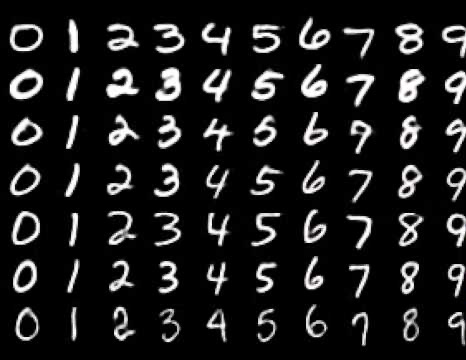
\includegraphics[width=0.5\textwidth]{images/mnist.png}
\caption{Alcune immagini del dataset MNIST: cifre scritte a mano da 0 a 9, in scala di grigi, di $28 \times 28$ pixel ciascuna.}
\label{fig:mnist}
\end{figure}

L'approccio più semplice è usare un MLP. L'immagine viene ``srotolata'' da una matrice $28 \times 28$ a un vettore $784 \times 1$, che diventa l'input di una rete con un hidden layer da 500 neuroni e un output layer da 10 neuroni, uno per classe (figura~\ref{fig:mlp-mnist}). La rete calcola:
\[
h(x, \vartheta) = \vartheta_h\, f(\vartheta_f x + b_f) + b_h
\]
dove $\vartheta_f \in \mathbb{R}^{500 \times 784}$, $b_f \in \mathbb{R}^{500}$, $\vartheta_h \in \mathbb{R}^{10 \times 500}$ e $b_h \in \mathbb{R}^{10}$. Quanti parametri ha? Basta sommare le dimensioni:
\[
500 \cdot 784 + 500 + 10 \cdot 500 + 10 = 397\,510.
\]

Un MLP così costruito funziona, ma quasi 400 mila parametri per immagini di $28 \times 28$ pixel sono tanti. Inoltre la rete tratta ogni pixel come una feature indipendente: la struttura spaziale dell'immagine va persa quando la srotoliamo.

\begin{figure}[htbp]
\centering
\begin{tikzpicture}[>=Stealth, font=\scriptsize,
  layer/.style={draw=Accent, fill=Accent!70, text=white, minimum width=6mm}]
  \node (img) at (0,0) {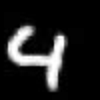
\includegraphics[width=8mm]{images/mnist-4.png}};
  \node[layer, minimum height=3.2cm] (l1) at (1.5,0) {\rotatebox{90}{784}};
  \node[layer, minimum height=2.0cm] (l2) at (3.6,0) {\rotatebox{90}{500}};
  \node[layer, minimum height=1.0cm] (l3) at (5.7,0) {\rotatebox{90}{10}};
  \draw[->] (img) -- (l1);
  \draw[->] (l1) -- node[above] {$\vartheta_f, b_f$} (l2);
  \draw[->] (l2) -- node[above] {$\vartheta_h, b_h$} (l3);
  \node[TextGray] at (1.5,-1.9) {input};
  \node[TextGray] at (3.6,-1.9) {hidden layer};
  \node[TextGray] at (5.7,-1.9) {output};
\end{tikzpicture}
\caption{Un MLP per MNIST: l'immagine $28 \times 28$ viene srotolata in un vettore di 784 valori, seguito da un hidden layer con 500 neuroni e da un output layer con 10 neuroni, uno per cifra.}
\label{fig:mlp-mnist}
\end{figure}

\section{Convolutional Neural Network}
Le Convolutional Neural Network sono progettate per far scalare le reti neurali a immagini molto grandi e a sequenze video. L'idea principale è \textbf{sostituire la moltiplicazione matriciale con la convoluzione} (figura~\ref{fig:cnn-pipeline}).

\begin{figure}[htbp]
\centering
\begin{tikzpicture}[>=Stealth, font=\scriptsize,
  blk/.style={draw=Accent, fill=Accent!70, text=white, minimum width=2.1cm, minimum height=0.9cm}]
  \node[blk, draw=LemmaColor, fill=LemmaColor!70] (in) at (0,0) {Input Image};
  \node[blk] (c1) at (2.9,0) {Convolution};
  \node[blk] (c2) at (5.8,0) {Convolution};
  \node (dots) at (7.9,0) {$\cdots$};
  \draw[->] (in) -- (c1);
  \draw[->] (c1) -- (c2);
  \draw[->] (c2) -- (dots);
\end{tikzpicture}
\caption{L'idea alla base di una CNN: l'immagine in input attraversa una sequenza di convoluzioni, che prendono il posto delle moltiplicazioni matriciali di un MLP.}
\label{fig:cnn-pipeline}
\end{figure}

\begin{osservazione}[Invarianza alla traslazione]
L'estrazione delle feature dovrebbe essere \textbf{invariante alla traslazione} lungo gli assi $x$ e $y$. Pensiamo all'esempio di MNIST: un 7 resta un 7 sia che si trovi al centro dell'immagine, sia che sia spostato di qualche pixel. Una moltiplicazione matriciale imparerebbe pesi diversi in posizioni diverse, mentre la convoluzione, come vedremo, applica gli stessi pesi in tutte le posizioni e mantiene questa invarianza.
\end{osservazione}

In altre parole, una CNN impara un certo numero di \textbf{filtri}, e li impara in modo che siano i migliori per risolvere il problema dato.

\subsection{Architettura e componenti}
Una CNN è una sequenza di layer, ognuno con i propri pesi $W_l$: prima alcuni layer convoluzionali, poi alcuni layer fully connected, che restituiscono la classe (figura~\ref{fig:cnn-arch}).

\begin{figure}[htbp]
\centering
\begin{tikzpicture}[>=Stealth, font=\scriptsize,
  conv/.style={draw, minimum width=5mm, minimum height=1.5cm, inner sep=1pt},
  fc/.style={draw, minimum width=7mm, minimum height=1.5cm, inner sep=1pt}]
  \node[draw, fill=TextGray!15, minimum width=1.1cm, minimum height=1.1cm, align=center] (in) at (0,0) {immagine};
  \foreach \k in {1,...,5} \node[conv] (C\k) at (0.4+1.0*\k,0) {$C_\k$};
  \foreach \k in {6,7,8} \node[fc] (F\k) at (0.6+1.05*\k,0) {$f_\k$};
  \node[draw=ObsColor, fill=ObsColor!15, rounded corners=4pt, minimum height=6mm] (out) at (10.8,0) {bike};
  \draw[->] (in) -- (C1);
  \foreach \a/\b in {C1/C2, C2/C3, C3/C4, C4/C5, C5/F6, F6/F7, F7/F8, F8/out} \draw[->] (\a) -- (\b);
  \foreach \k in {1,...,5} \draw[<-] (C\k.south) -- ++(0,-0.6) node[below] {$W_\k$};
  \foreach \k in {6,7,8} \draw[<-] (F\k.south) -- ++(0,-0.6) node[below] {$W_\k$};
\end{tikzpicture}
\caption{Architettura di una CNN (da \cite{Krizhevsky2012}): cinque layer convoluzionali $C_1, \dots, C_5$ e tre layer fully connected $f_6, f_7, f_8$, ciascuno con i propri pesi $W_l$. L'output è la classe dell'immagine in input, nell'esempio una bicicletta.}
\label{fig:cnn-arch}
\end{figure}

I layer convoluzionali sono costruiti combinando alcuni blocchi elementari (figura~\ref{fig:cnn-blocchi}):
\begin{itemize}
    \item \textbf{Filtri lineari 3D}: $y = F * x + b$, dove $F$ è un banco di filtri e $b$ il bias. È la convoluzione vera e propria, oggetto di questo capitolo.
    \item \textbf{ReLU}: $y = \max\{0, x\}$, la non linearità applicata dopo la convoluzione.
    \item \textbf{Downsampling}: riduce la dimensione spaziale dell'input.
    \item \textbf{Normalizzazione}: normalizza le risposte su gruppi di canali con una finestra scorrevole (sliding $\ell^2$).
    \item \textbf{Spatial pooling}: $y_{ijk} = \max_{pq \in \Omega_{ij}} x_{pqk}$, ovvero per ogni canale $k$ si prende il massimo in un intorno $\Omega_{ij}$ della posizione $(i, j)$.
\end{itemize}
Gli ultimi quattro blocchi li vedremo nella sezione~\ref{sec:cnn-layer}.

\begin{figure}[htbp]
\centering
\begin{tikzpicture}[>=Stealth, font=\scriptsize,
  box/.style={draw, minimum width=1.3cm, minimum height=0.8cm, align=center}]
  \foreach \nm/\xx/\yy/\content/\formula in {
      lin/0/0/{$(F, b)$}/{$y = F * x + b$},
      down/6.6/0/{$\downarrow$}/{$y$},
      relu/0/-1.5/{}/{$y = \max\{0, x\}$},
      norm/6.6/-1.5/{sliding $\ell^2$}/{$y$},
      pool/0/-3/{$\max$}/{$y_{ijk} = \max_{pq \in \Omega_{ij}} x_{pqk}$}} {
    \node[box] (\nm) at (\xx,\yy) {\content};
    \draw[->] ([xshift=-0.7cm]\nm.west) node[left] {$x$} -- (\nm.west);
    \draw[->] (\nm.east) -- ++(0.7,0) node[right] {\formula};
  }
  \draw[->, TextGray] ([xshift=-0.45cm, yshift=-0.2cm]relu.center) -- ([xshift=0.5cm, yshift=-0.2cm]relu.center);
  \draw[->, TextGray] ([yshift=-0.35cm]relu.center) -- ([yshift=0.35cm]relu.center);
  \draw[very thick, Accent] ([xshift=-0.4cm, yshift=-0.2cm]relu.center) -- ([yshift=-0.2cm]relu.center) -- ([xshift=0.4cm, yshift=0.25cm]relu.center);
  \foreach \nm/\lab in {lin/filtri lineari 3D, down/downsampling, relu/ReLU, norm/normalizzazione, pool/spatial pooling}
    \node[TextGray, above] at (\nm.north) {\lab};
\end{tikzpicture}
\caption{I blocchi elementari dei layer convoluzionali: filtri lineari 3D, downsampling, ReLU, normalizzazione e spatial pooling. Ciascun blocco riceve un input $x$ e restituisce un output $y$.}
\label{fig:cnn-blocchi}
\end{figure}

\subsection{La convoluzione 2D}
Partiamo da un esempio (figura~\ref{fig:cane}). Applichiamo a un'immagine in scala di grigi il kernel $[1, -1]$: ogni pixel dell'output è la differenza tra un pixel dell'input e il suo vicino a destra. Nelle zone uniformi la differenza è circa 0, e infatti l'output è grigio. Dove l'intensità cambia bruscamente in orizzontale, invece, la differenza è grande: l'output mette in evidenza i \textbf{bordi verticali} dell'immagine. Un kernel, quindi, risponde a una particolare caratteristica dell'input.

\begin{figure}[htbp]
\centering
\begin{tikzpicture}[>=Stealth, font=\small]
  \node (in) at (0,0) {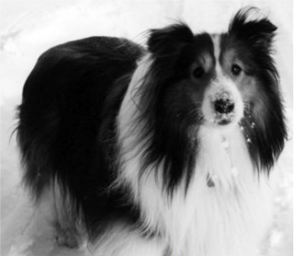
\includegraphics[width=4cm]{images/cnn-dog-input.png}};
  \node[below=0pt of in] {Input};
  \node (out) at (7.2,-1.1) {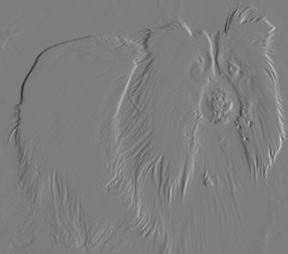
\includegraphics[width=4cm]{images/cnn-dog-output.png}};
  \node[below=0pt of out] {Output};
  \node[draw=Accent, minimum size=7mm] (k1) at (-0.35,-3.2) {$1$};
  \node[draw=Accent, minimum size=7mm, right=0pt of k1] (k2) {$-1$};
  \node[below=2pt of k1.south east] {Kernel};
  \draw[->, thick] (in.east) -- (out.west);
  \draw[->, thick] (k2.east) -- (out.west);
\end{tikzpicture}
\caption{Esempio di convoluzione 2D (da \cite{Goodfellow-et-al-2016}): il kernel $[1, -1]$ sottrae a ogni pixel il suo vicino a destra. Le zone uniformi diventano grigie, mentre i bordi verticali del cane vengono messi in evidenza.}
\label{fig:cane}
\end{figure}

In un layer possiamo imparare \textbf{più di un kernel}, in modo simile a quanto accade quando mettiamo più percettroni nello stesso layer di un MLP. Ogni kernel produce la propria uscita, e i layer successivi ricevono le uscite di tutti i kernel del layer precedente (figura~\ref{fig:multi-kernel}).

\begin{figure}[htbp]
\centering
\begin{tikzpicture}[>=Stealth, font=\scriptsize,
  blk/.style={draw=Accent, fill=Accent!70, text=white, minimum width=2.1cm, minimum height=0.9cm}]
  \node[blk, draw=LemmaColor, fill=LemmaColor!70] (in) at (0,0) {Input Image};
  \node[blk] (a1) at (3.2,0.75) {Convolution};
  \node[blk] (a2) at (3.2,-0.75) {Convolution};
  \node[blk] (b1) at (6.4,0.75) {Convolution};
  \node[blk] (b2) at (6.4,-0.75) {Convolution};
  \node (dots) at (8.6,0) {$\cdots$};
  \foreach \a in {a1,a2} \draw[->] (in.east) -- (\a.west);
  \foreach \a in {a1,a2} \foreach \b in {b1,b2} \draw[->] (\a.east) -- (\b.west);
\end{tikzpicture}
\caption{Più kernel per layer: ogni layer impara due convoluzioni, e ognuna di quelle del secondo layer riceve le uscite di entrambe quelle del primo.}
\label{fig:multi-kernel}
\end{figure}

\paragraph{Cross-correlation.}
I pesi da apprendere in un layer convoluzionale sono \textbf{i valori del kernel}. Consideriamo la figura~\ref{fig:cross-corr}: l'input è una matrice $3 \times 4$ e il kernel una matrice $2 \times 2$. Il kernel scorre sull'input e, in ogni posizione, moltiplica elemento per elemento i valori sovrapposti e li somma. Ad esempio, nella prima posizione l'output vale $aw + bx + ey + fz$. Il kernel ha solo 4 pesi, e questi restano 4 qualunque sia la dimensione dell'input.

\begin{figure}[htbp]
\centering
\begin{tikzpicture}[>=Stealth, font=\scriptsize]
  % input
  \node[TextGray] at (1.2,0.3) {Input};
  \numgrid[draw=Accent]{(0,0)}{0.6}{{a,b,c,d},{e,f,g,h},{i,j,k,l}}
  \cellrect[very thick, red!70!black]{(0,0)}{0.6}{0}{0}{2}{2}
  % kernel
  \node[TextGray] at (3.9,0.3) {Kernel};
  \numgrid[draw=Accent]{(3.3,0)}{0.6}{{w,x},{y,z}}
  % output
  \node[TextGray, anchor=east] at (0.1,-3.6) {Output};
  \foreach \rr/\cc/\sopra/\sotto in {0/0/aw + bx/ey + fz, 0/1/bw + cx/fy + gz, 0/2/cw + dx/gy + hz,
                                     1/0/ew + fx/iy + jz, 1/1/fw + gx/jy + kz, 1/2/gw + hx/ky + lz}
    \node[draw=Accent, minimum width=1.6cm, minimum height=0.9cm, align=center, anchor=north west]
      (o\rr\cc) at (0.2+1.75*\cc,-2.6-1.05*\rr) {$\sopra\, +$ \\ $\sotto$};
  \draw[very thick, red!70!black] (o00.north west) rectangle (o00.south east);
  \draw[->, red!70!black] (0.6,-1.2) -- (o00.north);
  \draw[->, red!70!black] (3.9,-1.2) to[out=-90, in=30] (o00.north east);
\end{tikzpicture}
\caption{Cross-correlation 2D (da \cite{Goodfellow-et-al-2016}): un kernel $2 \times 2$ scorre su un input $3 \times 4$ e produce un output $2 \times 3$. In rosso la prima posizione del kernel e il valore corrispondente dell'output. I pesi da apprendere sono soltanto i 4 valori del kernel.}
\label{fig:cross-corr}
\end{figure}

Formalizziamo. Sia $F$ l'immagine in input e $h$ un kernel di dimensione $(2k+1) \times (2k+1)$, con indici che vanno da $-k$ a $k$. La \textbf{cross-correlation} si definisce come:
\[
G = h \otimes F, \qquad G[i, j] = \sum_{u=-k}^{k}\sum_{v=-k}^{k} h[u, v]\, F[i + u, j + v]
\]
mentre la \textbf{convoluzione} si definisce come:
\[
G = h * F, \qquad G[i, j] = \sum_{u=-k}^{k}\sum_{v=-k}^{k} h[u, v]\, F[i - u, j - v]
\]
dove $G$ è l'output. L'unica differenza è il segno degli indici: la convoluzione equivale a una cross-correlation con il kernel \textbf{ribaltato} su entrambi gli assi, ovvero ruotato di $180^\circ$ (figura~\ref{fig:flip}).

\begin{figure}[htbp]
\centering
\begin{tikzpicture}[font=\small]
  \foreach \xx/\lab/\vals in {0/{Kernel $F$}/{{a,b,c},{d,e,f},{g,h,i}}, 4.2/{Kernel ribaltato}/{{i,h,g},{f,e,d},{c,b,a}}} {
    \numgrid[draw=Accent, font=\small]{(\xx,0)}{0.6}{\vals}
    \foreach \lb [count=\cc from 0] in {-1,0,1} {
      \node[font=\scriptsize, TextGray] at (\xx+0.3+0.6*\cc,0.25) {$\lb$};
      \node[font=\scriptsize, TextGray] at (\xx-0.3,-0.3-0.6*\cc) {$\lb$};
    }
    \node at (\xx+0.9,-2.15) {\lab};
  }
  \draw[->, thick, Accent] (2.1,-0.9) -- (3.7,-0.9) node[midway, above, font=\scriptsize] {$180^\circ$};
\end{tikzpicture}
\caption{A sinistra un kernel $3 \times 3$ con indici da $-1$ a $1$, a destra lo stesso kernel ribaltato su entrambi gli assi. Calcolare la convoluzione con il kernel di sinistra equivale a calcolare la cross-correlation con quello di destra.}
\label{fig:flip}
\end{figure}

\begin{osservazione}
Quella che nelle CNN chiamiamo convoluzione è in realtà, quasi sempre, una cross-correlation, come in figura~\ref{fig:cross-corr}. Nella pratica la differenza non conta: i valori del kernel vengono appresi, per cui una rete che usa la convoluzione imparerebbe semplicemente il kernel ribaltato.
\end{osservazione}

\paragraph{Esempio.}
Consideriamo l'immagine $5 \times 5$ in scala di grigi della figura~\ref{fig:sharpen}, divisa in una zona chiara (valore 2) e una scura (valore 8). Le applichiamo il kernel di \emph{sharpening}:
\[
K = \begin{bmatrix} 0 & -1 & 0 \\ -1 & 5 & -1 \\ 0 & -1 & 0 \end{bmatrix}.
\]
Calcoliamo l'output della cross-correlation, facendo scorrere il kernel solo nelle posizioni in cui sta tutto dentro l'immagine.

\textbf{Soluzione.} Le posizioni possibili sono $3 \times 3$, quindi l'output è una matrice $3 \times 3$. Nella prima posizione il kernel copre una zona uniforme, tutta di valore 2, e restituisce $5 \cdot 2 - 4 \cdot 2 = 2$: le zone uniformi restano invariate. Nella seconda posizione (in rosso in figura) il pixel centrale vale 2, mentre il suo vicino a destra vale 8:
\[
G[0, 1] = 5 \cdot 2 - (2 + 2 + 8 + 2) = -4.
\]

Spostandoci di un'altra posizione il centro vale 8 e il vicino a sinistra 2, per cui $G[0, 2] = 5 \cdot 8 - (8 + 2 + 8 + 8) = 14$. Il salto tra le due zone, che nell'input era da 2 a 8, nell'output diventa da $-4$ a 14: il kernel accentua i bordi, ed è proprio questo che rende l'immagine più nitida.

\begin{figure}[htbp]
\centering
\begin{tikzpicture}[font=\scriptsize]
  \def\csz{0.5}
  % input con sfondo proporzionale al valore
  \foreach \row [count=\ri from 0] in {{2,2,2,8,8},{2,2,2,8,8},{2,2,2,8,8},{2,2,8,8,8},{2,2,8,8,8}} {
    \foreach \v [count=\ci from 0] in \row {
      \pgfmathtruncatemacro\sh{8*\v}
      \pgfmathtruncatemacro\tv{100*(\v<6)}
      \node[draw=TextGray, minimum size=\csz cm, inner sep=0pt, anchor=north west, fill=black!\sh, text=black!\tv]
        at ({\ci*\csz},{-\ri*\csz}) {$\v$};
    }
  }
  \cellrect[very thick, red!70!black]{(0,0)}{\csz}{1}{0}{3}{3}
  \node at (1.25,0.3) {Input};
  \node[font=\large] at (2.95,-1.25) {$\otimes$};
  \numgrid[draw=Accent, minimum size=0.5cm]{(3.4,-0.5)}{\csz}{{0,-1,0},{-1,5,-1},{0,-1,0}}
  \node at (4.15,-0.2) {Kernel};
  \node[font=\large] at (5.35,-1.25) {$=$};
  % output, con sfondo proporzionale al valore (limitato tra 0 e 10)
  \foreach \row [count=\ri from 0] in {{2,-4,14},{2,-10,14},{-4,20,8}} {
    \foreach \v [count=\ci from 0] in \row {
      \pgfmathtruncatemacro\sh{8*min(max(\v,0),10)}
      \pgfmathtruncatemacro\tv{100*(\v<6)}
      \node[draw=TextGray, minimum size=\csz cm, inner sep=0pt, anchor=north west, fill=black!\sh, text=black!\tv, font=\tiny]
        at ({5.8+\ci*\csz},{-0.5-\ri*\csz}) {$\v$};
    }
  }
  \cellrect[very thick, red!70!black]{(5.8,-0.5)}{\csz}{1}{0}{1}{1}
  \node at (6.55,-0.2) {Output};
\end{tikzpicture}
\caption{Il kernel di sharpening applicato a un'immagine $5 \times 5$. Il colore delle celle segue il valore (i valori negativi sono resi in bianco, come se fossero 0). In rosso la seconda posizione del kernel e il valore corrispondente dell'output, $-4$: lungo il bordo tra le due zone il contrasto aumenta.}
\label{fig:sharpen}
\end{figure}

\subsection{Convoluzione 3D, padding, dilation e stride}
La forma dell'output di un layer convoluzionale dipende dalla forma del suo input e da alcune scelte: la forma del kernel, lo \textbf{zero padding}, la \textbf{dilation} e lo \textbf{stride}. In ogni caso valgono tre cose:
\begin{itemize}
    \item i pesi del layer corrispondono ai valori del kernel.
    \item i pesi sono \textbf{condivisi} all'interno di un canale (depth slice), ovvero lo stesso kernel viene usato in tutte le posizioni.
    \item stiamo di fatto imparando dei filtri che rispondono a parti, entità o indizi visivi dell'immagine.
\end{itemize}

\paragraph{Convoluzione 3D.}
Un'immagine a colori non è una matrice ma un \textbf{volume}: ad esempio un'immagine RGB ha 3 canali, per cui ha dimensione $W \times H \times 3$. In questo caso il kernel ha la stessa profondità dell'input: con un input di $C$ canali, un filtro $F \times F$ ha dimensione $F \times F \times C$. In ogni posizione il filtro calcola la cross-correlation su ciascun canale, somma i risultati e aggiunge il bias, producendo \textbf{un solo valore}. Ogni filtro produce quindi una matrice 2D, e con $K$ filtri l'output ha profondità $K$.

\paragraph{Esempio.}
Consideriamo un input $5 \times 5 \times 3$, a cui aggiungiamo un bordo di zeri ottenendo un volume $7 \times 7 \times 3$, e due filtri $W_0$ e $W_1$ di dimensione $3 \times 3 \times 3$, con bias $b_0 = 1$ e $b_1 = 0$. I filtri si spostano di 2 posizioni alla volta. Calcoliamo il primo valore dell'output del filtro $W_0$.

\textbf{Soluzione.} Il filtro $W_0$ si sovrappone all'angolo in alto a sinistra dei tre canali (in figura~\ref{fig:conv3d}, i riquadri blu). Per ciascun canale calcoliamo la cross-correlation tra la porzione $3 \times 3$ dell'input e il canale corrispondente del filtro, ottenendo rispettivamente 2, 1 e 2. Sommando i tre contributi e il bias:
\[
o[0, 0, 0] = 2 + 1 + 2 + b_0 = 2 + 1 + 2 + 1 = 6.
\]
Ripetendo il calcolo in tutte le posizioni si ottiene una matrice $3 \times 3$. Facendo lo stesso con $W_1$ se ne ottiene un'altra. L'output ha quindi dimensione $3 \times 3 \times 2$, una matrice per filtro.

\begin{figure}[htbp]
\centering
\begin{tikzpicture}[font=\tiny]
  \def\csz{0.4}
  \tikzset{gcell/.style={minimum size=0.4cm, font=\tiny}}
  % input
  \foreach \cc/\vals in {
      0/{{0,0,0,0,0,0,0},{0,2,1,2,2,1,0},{0,2,2,0,0,0,0},{0,0,2,2,0,1,0},{0,2,0,2,0,1,0},{0,2,0,1,0,2,0},{0,0,0,0,0,0,0}},
      1/{{0,0,0,0,0,0,0},{0,0,2,1,1,1,0},{0,1,1,1,2,2,0},{0,2,2,1,1,2,0},{0,1,0,2,0,2,0},{0,1,0,0,1,0,0},{0,0,0,0,0,0,0}},
      2/{{0,0,0,0,0,0,0},{0,0,1,2,1,2,0},{0,2,2,1,1,1,0},{0,0,1,1,0,2,0},{0,0,0,0,2,2,0},{0,2,0,2,1,1,0},{0,0,0,0,0,0,0}}} {
    \node[font=\scriptsize, anchor=south west] at (0,-3.35*\cc) {$x[:,:,\cc]$};
    \numgrid[gcell, fill=Accent!6]{(0,-3.35*\cc)}{\csz}{\vals}
    \cellrect[very thick, blue!70!black]{(0,-3.35*\cc)}{\csz}{0}{0}{3}{3}
  }
  % filtri
  \foreach \w/\xx/\vals in {
      0/3.4/{{{-1,0,1},{0,-1,0},{-1,1,1}},{{-1,0,1},{1,1,0},{-1,1,0}},{{-1,-1,0},{1,0,0},{1,1,0}}},
      1/5.1/{{{0,0,-1},{-1,0,0},{0,-1,-1}},{{-1,0,1},{0,0,0},{1,0,0}},{{0,0,0},{0,0,1},{1,-1,0}}}} {
    \foreach \m [count=\cc from 0] in \vals {
      \node[font=\scriptsize, anchor=south west] at (\xx,-3.35*\cc) {$W_\w[:,:,\cc]$};
      \numgrid[gcell, fill=red!8]{(\xx,-3.35*\cc)}{\csz}{\m}
    }
  }
  \node[font=\scriptsize, anchor=south west] at (3.4,-8.5) {$b_0 = 1$};
  \node[font=\scriptsize, anchor=south west] at (5.1,-8.5) {$b_1 = 0$};
  \cellrect[very thick, red!70!black]{(3.4,0)}{\csz}{0}{0}{3}{3}
  \cellrect[very thick, red!70!black]{(3.4,-3.35)}{\csz}{0}{0}{3}{3}
  \cellrect[very thick, red!70!black]{(3.4,-6.7)}{\csz}{0}{0}{3}{3}
  % output
  \foreach \cc/\vals in {0/{{6,4,5},{7,3,6},{0,0,-3}}, 1/{{-5,2,0},{-2,-3,-3},{0,1,0}}} {
    \node[font=\scriptsize, anchor=south west] at (6.9,-3.35*\cc) {$o[:,:,\cc]$};
    \numgrid[gcell, fill=LemmaColor!12]{(6.9,-3.35*\cc)}{\csz}{\vals}
  }
  \cellrect[very thick, LemmaColor]{(6.9,0)}{\csz}{0}{0}{1}{1}
  \node[font=\scriptsize, TextGray, align=center] at (1.4,-10.0) {input $7 \times 7 \times 3$\\(con padding)};
  \node[font=\scriptsize, TextGray, align=center] at (4.8,-9.0) {filtri $3 \times 3 \times 3$};
  \node[font=\scriptsize, TextGray, align=center] at (7.5,-5.1) {output\\$3 \times 3 \times 2$};
\end{tikzpicture}
\caption{Una convoluzione 3D con due filtri e stride 2. A sinistra i tre canali dell'input, già circondati da un bordo di zeri. Al centro i tre canali dei filtri $W_0$ e $W_1$ con i rispettivi bias, a destra le due matrici dell'output, una per filtro. In blu la porzione di input coperta da $W_0$ (in rosso) nella prima posizione, in verde il valore corrispondente $o[0,0,0] = 6$.}
\label{fig:conv3d}
\end{figure}

\paragraph{Padding.}
Applicando un kernel $3 \times 3$ a un'immagine $5 \times 5$, come nell'esempio dello sharpening, l'output si è ridotto a $3 \times 3$: il kernel non può centrarsi sui pixel del bordo. Per evitarlo si usa lo \textbf{zero padding}, ovvero si aggiungono $P$ bordi di zeri attorno all'input (figura~\ref{fig:padding}). Ad esempio, un input di $32 \times 32 \times 3$ con due bordi di zeri ($P = 2$) diventa un volume di $36 \times 36 \times 3$. Applicando tre filtri $5 \times 5 \times 3$ con passo 1, si ottiene un output di $32 \times 32 \times 3$: la dimensione spaziale dell'input viene preservata.

\begin{figure}[htbp]
\centering
\begin{tikzpicture}[>=Stealth, font=\scriptsize]
  \def\csz{0.375}
  % input con padding P = 1
  \fill[Accent!25] (\csz,-\csz) rectangle (6*\csz,-6*\csz);
  \emptygrid[TextGray, dashed]{(0,0)}{\csz}{7}{7}
  \emptygrid[TextGray]{(\csz,-\csz)}{\csz}{5}{5}
  \foreach \i in {0,...,6} \foreach \j in {0,...,6} {
    \pgfmathtruncatemacro\bordo{(\i==0)||(\i==6)||(\j==0)||(\j==6)}
    \ifnum\bordo=1 \node[TextGray] at ({(\j+0.5)*\csz},{-(\i+0.5)*\csz}) {0}; \fi
  }
  \cellrect[very thick, red!70!black]{(0,0)}{\csz}{0}{0}{3}{3}
  \node at (1.3125,0.3) {input $5 \times 5$, $P = 1$};
  % output
  \fill[LemmaColor!30] (4.2,-\csz) rectangle (4.2+5*\csz,-6*\csz);
  \emptygrid[TextGray]{(4.2,-\csz)}{\csz}{5}{5}
  \cellrect[very thick, red!70!black, fill=red!25]{(4.2,-\csz)}{\csz}{0}{0}{1}{1}
  \node at (5.1375,0.3) {output $5 \times 5$};
  \draw[->, thick] (2.9,-1.3125) -- (4.0,-1.3125);
\end{tikzpicture}
\caption{Zero padding (si veda \cite{Dumoulin2016}): un input $5 \times 5$ (in verde petrolio) viene circondato da un bordo di zeri ($P = 1$). Un kernel $3 \times 3$ con passo 1, di cui in rosso è riportata la prima posizione, produce un output $5 \times 5$, della stessa dimensione dell'input.}
\label{fig:padding}
\end{figure}

\paragraph{Stride.}
Lo \textbf{stride} $S$ è il passo con cui il kernel si sposta sull'input. Con $S = 1$ il kernel si sposta di una cella alla volta, mentre con $S = 2$ salta una posizione ogni volta, e l'output si riduce. Ad esempio, un kernel $3 \times 3$ su un input $7 \times 7$ produce un output $5 \times 5$ con $S = 1$, e un output $3 \times 3$ con $S = 2$ (figura~\ref{fig:stride}).

\begin{figure}[htbp]
\centering
\begin{tikzpicture}[font=\scriptsize]
  \def\csz{0.375}
  \foreach \yy/\S/\nout in {0/1/5, -3.4/2/3} {
    \begin{scope}[yshift=\yy cm]
      \fill[Accent!25] (0,0) rectangle (7*\csz,-7*\csz);
      \emptygrid[TextGray]{(0,0)}{\csz}{7}{7}
      \node[anchor=east, align=right] at (-0.2,-1.3125) {$S = \S$};
      % output
      \fill[LemmaColor!30] (4.0,0) rectangle (4.0+\nout*\csz,-\nout*\csz);
      \emptygrid[TextGray]{(4.0,0)}{\csz}{\nout}{\nout}
      \node[anchor=west] at (4.1+\nout*\csz,-0.5*\nout*\csz) {output $\nout \times \nout$};
    \end{scope}
  }
  % S = 1: due posizioni consecutive
  \cellrect[very thick, red!70!black]{(0,0)}{\csz}{0}{0}{3}{3}
  \cellrect[very thick, LemmaColor!70!black]{(0.04,-0.04)}{\csz}{1}{0}{3}{3}
  \cellrect[fill=red!60]{(4.0,0)}{\csz}{0}{0}{1}{1}
  \cellrect[fill=LemmaColor!80!black]{(4.0,0)}{\csz}{1}{0}{1}{1}
  % S = 2: tre posizioni
  \begin{scope}[yshift=-3.4cm]
    \cellrect[very thick, red!70!black]{(0,0)}{\csz}{0}{0}{3}{3}
    \cellrect[very thick, LemmaColor!70!black]{(0.04,-0.04)}{\csz}{2}{0}{3}{3}
    \cellrect[very thick, blue!70!black]{(-0.04,0.04)}{\csz}{0}{2}{3}{3}
    \cellrect[fill=red!60]{(4.0,0)}{\csz}{0}{0}{1}{1}
    \cellrect[fill=LemmaColor!80!black]{(4.0,0)}{\csz}{1}{0}{1}{1}
    \cellrect[fill=blue!60]{(4.0,0)}{\csz}{0}{1}{1}{1}
  \end{scope}
  \node at (1.3125,0.3) {input $7 \times 7$};
\end{tikzpicture}
\caption{Lo stride, con un kernel $3 \times 3$ su un input $7 \times 7$. In alto, con $S = 1$, la seconda posizione del kernel (in verde) è spostata di una cella rispetto alla prima (in rosso) e l'output è $5 \times 5$. In basso, con $S = 2$, il kernel si sposta di due celle sia in orizzontale (in verde) sia in verticale (in blu), e l'output si riduce a $3 \times 3$. Ogni colore indica la posizione del kernel e il valore dell'output che produce.}
\label{fig:stride}
\end{figure}

\paragraph{Dilation.}
Con la \textbf{dilation} gli elementi del kernel non sono più adiacenti, ma distanziati: con un fattore di dilation $d$ tra un elemento e l'altro restano $d - 1$ celle libere. Un kernel $3 \times 3$ con $d = 2$, ad esempio, copre un'area di $5 \times 5$ pur avendo sempre 9 pesi (figura~\ref{fig:dilation}).

In generale, un kernel di lato $F$ con dilation $d$ copre un'area di lato
\[
F + (F - 1)(d - 1).
\]
Il punto più importante è che le convoluzioni dilatate permettono un'espansione esponenziale del receptive field (la porzione di input che influenza un valore dell'output) senza perdere risoluzione né copertura. Si ottiene quindi un receptive field più ampio con lo stesso costo in calcolo e in memoria.

\begin{figure}[htbp]
\centering
\begin{tikzpicture}[>=Stealth, font=\scriptsize]
  \def\csz{0.375}
  \fill[Accent!25] (0,0) rectangle (7*\csz,-7*\csz);
  \foreach \i in {0,2,4} {\foreach \j in {0,2,4} {\cellrect[fill=Accent!80]{(0,0)}{\csz}{\j}{\i}{1}{1}}}
  \emptygrid[TextGray]{(0,0)}{\csz}{7}{7}
  \cellrect[very thick, dashed, red!70!black]{(0,0)}{\csz}{0}{0}{5}{5}
  \node at (1.3125,0.3) {input $7 \times 7$};
  \fill[LemmaColor!30] (4.2,-\csz) rectangle (4.2+3*\csz,-4*\csz);
  \emptygrid[TextGray]{(4.2,-\csz)}{\csz}{3}{3}
  \cellrect[very thick, red!70!black, fill=red!25]{(4.2,-\csz)}{\csz}{0}{0}{1}{1}
  \node at (4.7625,0.3) {output $3 \times 3$};
  \draw[->, thick] (2.9,-1.3125) -- (4.0,-1.3125);
\end{tikzpicture}
\caption{Convoluzione dilatata (si veda \cite{Dumoulin2016}): un kernel $3 \times 3$ con $d = 2$ applicato a un input $7 \times 7$. Le celle scure sono quelle moltiplicate per i 9 pesi del kernel nella prima posizione, mentre il riquadro tratteggiato è l'area $5 \times 5$ che coprono. Con stride 1 l'output è $3 \times 3$.}
\label{fig:dilation}
\end{figure}

\subsection{Local receptive field e shared weights}
Vediamo ora da dove nasce il risparmio di parametri. In una rete neurale classica ogni nodo è \textbf{fully connected}, ovvero collegato a tutti i nodi del layer adiacente. Con un'immagine di $1000 \times 1000$ pixel, ogni neurone del primo hidden layer ha quindi un milione di parametri. Le CNN risolvono il problema con tre strumenti:
\begin{itemize}
    \item \textbf{Local receptive field}.
    \item \textbf{Shared weights}.
    \item \textbf{Pooling layer}, che riducono la dimensionalità man mano che si va in profondità (li vedremo nella sezione~\ref{subsec:pooling}).
\end{itemize}

\paragraph{Local receptive field.}
Ogni neurone di un hidden layer è collegato soltanto a una regione dell'input, detta \textbf{receptive field}, e non a tutta l'immagine. Ogni connessione serve ad apprendere un peso, per cui ogni nodo ha di fatto un proprio filtro. Ad esempio, con un receptive field di $5 \times 5$ ogni neurone ha 25 connessioni (figura~\ref{fig:receptive}, al centro).

\paragraph{Shared weights.}
Una feature può comparire in qualunque punto dell'immagine. Per questo motivo, i neuroni di uno stesso layer \textbf{condividono i pesi}: sono tutti sensibili alla stessa feature (la risposta del filtro), calcolata in posizioni diverse dell'input (figura~\ref{fig:receptive}, a destra). Una mappa di pesi applicata in posizioni diverse è esattamente una convoluzione.

\begin{figure}[htbp]
\centering
\begin{tikzpicture}[font=\scriptsize, neuron/.style={draw, circle, minimum size=4mm, inner sep=0pt}]
  \def\csz{0.25}
  % fully connected
  \fill[TextGray!20] (0,0) rectangle (8*\csz,-8*\csz);
  \emptygrid[white]{(0,0)}{\csz}{8}{8}
  \node[neuron] (n) at (3.0,-1.0) {};
  \foreach \i in {0,...,7} \foreach \j in {0,...,7}
    \draw[TextGray, very thin] ({(\j+0.5)*\csz},{-(\i+0.5)*\csz}) -- (n);
  \node[above] at (n.north) {$\vartheta$};
  \node at (1.5,-2.5) {fully connected};
  % local receptive field
  \begin{scope}[xshift=4.2cm]
    \fill[TextGray!20] (0,0) rectangle (8*\csz,-8*\csz);
    \emptygrid[white]{(0,0)}{\csz}{8}{8}
    \foreach \col/\cc/\rr/\yy in {red!70!black/1/0/-0.2, LemmaColor/4/2/-1.0, blue!70!black/1/5/-1.8} {
      \cellrect[very thick, draw=\col]{(0,0)}{\csz}{\cc}{\rr}{3}{3}
      \node[neuron, draw=\col] (m) at (3.0,\yy) {};
      \draw[draw=\col] ({\cc*\csz},{-\rr*\csz}) -- (m) -- ({(\cc+3)*\csz},{-(\rr+3)*\csz});
    }
    \node at (1.5,-2.5) {local receptive field};
  \end{scope}
  % shared weights
  \begin{scope}[xshift=8.4cm]
    \fill[TextGray!20] (0,0) rectangle (8*\csz,-8*\csz);
    \emptygrid[white]{(0,0)}{\csz}{8}{8}
    \foreach \cc/\rr/\yy in {1/0/-0.2, 4/2/-1.0, 1/5/-1.8} {
      \cellrect[very thick]{(0,0)}{\csz}{\cc}{\rr}{3}{3}
      \node[neuron] (m) at (3.0,\yy) {};
      \draw ({\cc*\csz},{-\rr*\csz}) -- (m) -- ({(\cc+3)*\csz},{-(\rr+3)*\csz});
      \node[right] at (m.east) {$\vartheta$};
    }
    \node at (1.5,-2.5) {shared weights};
  \end{scope}
\end{tikzpicture}
\caption{A sinistra, un neurone fully connected: ogni pixel dell'immagine è collegato al neurone con un proprio peso. Al centro, con il local receptive field ogni neurone vede solo una regione $3 \times 3$ dell'immagine, con i propri pesi (un colore per neurone). A destra, con gli shared weights tutti i neuroni usano gli stessi pesi $\vartheta$ in posizioni diverse: è una convoluzione.}
\label{fig:receptive}
\end{figure}

Torniamo al nostro esempio di MNIST. Nell'MLP ogni neurone dell'hidden layer aveva 784 pesi, uno per pixel, e il solo primo layer contava $500 \cdot 784 + 500 = 392\,500$ parametri. Un filtro $5 \times 5$, invece, ha 25 pesi più un bias, e questo numero non dipende dalla dimensione dell'immagine. Anche imparando 6 filtri diversi, il layer convoluzionale ha appena $6 \cdot (25 + 1) = 156$ parametri.

\subsection{Dimensione dell'output}
Mettendo insieme tutto quello che abbiamo visto, possiamo calcolare la dimensione dell'output di un layer convoluzionale. Siano:
\begin{itemize}
    \item $W \times H$ la dimensione dell'input.
    \item $F_w \times F_h$ la dimensione del kernel.
    \item $P$ la dimensione del padding.
    \item $S_w$ e $S_h$ lo stride rispettivamente in larghezza e in altezza.
\end{itemize}
La dimensione dell'output è:
\[
\text{output width} = \frac{W - F_w + 2P}{S_w} + 1, \qquad \text{output height} = \frac{H - F_h + 2P}{S_h} + 1.
\]
Con una dilation $d > 1$ basta sostituire alla dimensione del kernel quella dell'area che copre, $F + (F - 1)(d - 1)$.

Possiamo verificare la formula sulle figure precedenti. Per lo stride vale $(7 - 3 + 0)/2 + 1 = 3$ e per il padding $(5 - 3 + 2)/1 + 1 = 5$. Per la convoluzione 3D otteniamo $(5 - 3 + 2)/2 + 1 = 3$, e per la dilation $(7 - 5 + 0)/1 + 1 = 3$. Su MNIST, un filtro $5 \times 5$ senza padding e con stride 1 produce un output di $(28 - 5)/1 + 1 = 24$ pixel di lato, mentre con $P = 2$ la dimensione resta 28.

\begin{osservazione}
Se il risultato della formula non è un numero intero, il valore dello stride non è corretto. Ad esempio, con $W = 10$, $P = 0$, $F = 3$ e $S = 5$:
\[
\frac{W - F + 2P}{S} + 1 = \frac{10 - 3 + 0}{5} + 1 = \frac{7}{5} + 1
\]
che non è intero: il kernel non riesce a coprire l'input con passi regolari. Senza padding, lo stride può valere solo 1 o 7, gli unici divisori di 7. In questi casi lo zero padding ci viene in aiuto: con $S = 3$, ad esempio, basta $P = 1$ per ottenere $(10 - 3 + 2)/3 + 1 = 4$.
\end{osservazione}

\subsection{Un esempio reale: AlexNet}\label{subsec:alexnet}
Applichiamo la formula a una rete reale, \textbf{AlexNet} \cite{Krizhevsky2012}, ovvero la CNN di figura~\ref{fig:cnn-arch}. L'input è un'immagine RGB di $227 \times 227 \times 3$ pixel\footnote{Il paper e le slide riportano un input di $224 \times 224$, ma con questa dimensione la formula non restituisce un numero intero. I conti tornano con $227 \times 227$, che è la dimensione usata nelle implementazioni della rete.}. Il primo layer convoluzionale ha 96 filtri di $11 \times 11 \times 3$, con stride $S = 4$ e senza padding. La dimensione dell'output è quindi:
\[
\frac{227 - 11 + 0}{4} + 1 = 55
\]
ovvero ogni filtro produce una mappa di $55 \times 55$. Il primo layer ha $96 \cdot 11 \cdot 11 \cdot 3 = 34\,848$ pesi, più 96 bias (uno per filtro), mentre le unità di output sono $55 \cdot 55 \cdot 96 = 290\,400$.

La tabella~\ref{tab:alexnet} riporta gli stessi conti per tutti i layer. Il dato interessante è come si distribuiscono i pesi. I cinque layer convoluzionali hanno circa 2.3 milioni di pesi, meno del 4\% del totale, ma contano il 90\% delle connessioni (e quindi delle operazioni). I tre layer fully connected, al contrario, hanno quasi 59 milioni di pesi: è lì che si concentra la memoria occupata dalla rete.

\begin{table}[htbp]
\centering
\small
\begin{tabular}{@{}lrrr@{}}
\toprule
Layer & Unità & Pesi & Connessioni \\
\midrule
$L_1$ (conv) & 290\,400 & 34\,848 & 105\,415\,200 \\
$L_2$ (conv) & 186\,624 & 307\,200 & 111\,974\,400 \\
$L_3$ (conv) & 64\,896 & 884\,736 & 149\,520\,384 \\
$L_4$ (conv) & 64\,896 & 663\,552 & 112\,140\,288 \\
$L_5$ (conv) & 43\,264 & 442\,368 & 74\,760\,192 \\
$L_6$ (dense) & 4\,096 & 37\,748\,736 & 37\,748\,736 \\
$L_7$ (dense) & 4\,096 & 16\,777\,216 & 16\,777\,216 \\
$L_8$ (dense) & 1\,000 & 4\,096\,000 & 4\,096\,000 \\
\midrule
Totale conv & 650\,080 & 2\,332\,704 & 553\,810\,464 \\
Totale dense & 9\,192 & 58\,621\,952 & 58\,621\,952 \\
Totale & 659\,272 & 60\,954\,656 & 612\,432\,416 \\
\bottomrule
\end{tabular}
\caption{Unità, pesi e connessioni dei layer di AlexNet \cite{Krizhevsky2012}. I layer \emph{dense} sono i layer fully connected, e i pesi non includono i bias.}
\label{tab:alexnet}
\end{table}

\section{Sparse connections e parameter sharing}
Riprendiamo le idee di local receptive field e shared weights con lo schema di \cite{Goodfellow-et-al-2016}, in cui input e output sono vettori 1D. In questo modo è più semplice vedere quali connessioni ci sono e quali parametri vengono usati.

\subsection{Sparse connections}
In una rete fully connected ogni output dipende da tutti gli input. In un layer convoluzionale, invece, ogni output dipende solo dagli input coperti dal kernel: si parla quindi di \textbf{sparse connections} (connessioni sparse). Possiamo guardare la cosa da due punti di vista (figura~\ref{fig:sparse}):
\begin{itemize}
    \item \textbf{dal basso}: fissato un input, ad esempio $x_3$, con un kernel di larghezza 3 questo influenza solo tre output ($s_2$, $s_3$ e $s_4$). Con la moltiplicazione matriciale, invece, li influenza tutti.
    \item \textbf{dall'alto}: fissato un output, ad esempio $s_3$, questo dipende solo da tre input ($x_2$, $x_3$ e $x_4$). Questi input formano il \textbf{receptive field} di $s_3$.
\end{itemize}

\begin{figure}[htbp]
\centering
\begin{tikzpicture}[>=Stealth, font=\scriptsize,
  unit/.style={draw, circle, minimum size=6mm, inner sep=0pt}]
  % \md = 0: si guarda dal basso (input x_3), \md = 1: dall'alto (output s_3)
  % \fc = 0: convoluzione con kernel di larghezza 3, \fc = 1: fully connected
  \foreach \px/\py/\fc/\md in {0/0/0/0, 0/-2.4/1/0, 5.4/0/0/1, 5.4/-2.4/1/1} {
    \begin{scope}[shift={(\px,\py)}]
      \foreach \i in {1,...,5} {
        \pgfmathtruncatemacro\xon{((\md == 0) && (\i == 3)) || ((\md == 1) && ((\fc == 1) || (abs(\i - 3) <= 1)))}
        \pgfmathtruncatemacro\son{((\md == 1) && (\i == 3)) || ((\md == 0) && ((\fc == 1) || (abs(\i - 3) <= 1)))}
        \pgfmathtruncatemacro\xf{35*\xon}
        \pgfmathtruncatemacro\sff{35*\son}
        \node[unit, fill=TextGray!\xf] (x\i) at ({0.85*(\i-1)},0) {$x_\i$};
        \node[unit, fill=TextGray!\sff] (s\i) at ({0.85*(\i-1)},1.4) {$s_\i$};
      }
      \foreach \i in {1,...,5} {
        \foreach \j in {1,...,5} {
          \pgfmathtruncatemacro\e{(\fc == 1) || (abs(\i - \j) <= 1)}
          \ifnum\e=1 \draw[->, thin] (x\i) -- (s\j); \fi
        }
      }
    \end{scope}
  }
  \node at (1.7,2.1) {dal basso: l'input $x_3$};
  \node at (7.1,2.1) {dall'alto: l'output $s_3$};
  \node[left, align=right] at (-0.45,0.7) {convoluzione\\(kernel 3)};
  \node[left, align=right] at (-0.45,-1.7) {moltiplicazione\\matriciale};
\end{tikzpicture}
\caption{Sparse connections (da \cite{Goodfellow-et-al-2016}). A sinistra, le unità di output influenzate dall'input $x_3$: con un kernel di larghezza 3 sono solo tre, con la moltiplicazione matriciale sono tutte. A destra, le unità di input che influenzano l'output $s_3$, ovvero il suo receptive field.}
\label{fig:sparse}
\end{figure}

Il receptive field cresce man mano che si va in profondità (figura~\ref{fig:receptive-depth}). Un'unità del secondo layer, ad esempio $g_3$, è collegata direttamente solo a tre unità del layer precedente. Ognuna di queste, però, dipende a sua volta da tre input, per cui $g_3$ dipende indirettamente da tutti e cinque gli input. L'effetto aumenta se la rete usa lo stride o il pooling (sezione~\ref{subsec:pooling}). Quindi, anche se le connessioni dirette sono sparse, le unità dei layer più profondi possono essere collegate indirettamente a tutta l'immagine (o quasi).

\begin{figure}[htbp]
\centering
\begin{tikzpicture}[>=Stealth, font=\scriptsize,
  unit/.style={draw, circle, minimum size=6mm, inner sep=0pt}]
  \foreach \i in {1,...,5} {
    \pgfmathtruncatemacro\hf{35*(abs(\i - 3) <= 1)}
    \pgfmathtruncatemacro\gf{35*(\i == 3)}
    \node[unit, fill=TextGray!35] (x\i) at ({0.85*(\i-1)},0) {$x_\i$};
    \node[unit, fill=TextGray!\hf] (h\i) at ({0.85*(\i-1)},1.3) {$h_\i$};
    \node[unit, fill=TextGray!\gf] (g\i) at ({0.85*(\i-1)},2.6) {$g_\i$};
  }
  \foreach \i in {1,...,5} {
    \foreach \j in {1,...,5} {
      \pgfmathtruncatemacro\e{abs(\i - \j) <= 1}
      \ifnum\e=1 \draw[->, thin] (x\i) -- (h\j); \draw[->, thin] (h\i) -- (g\j); \fi
    }
  }
\end{tikzpicture}
\caption{Il receptive field delle unità nei layer profondi (da \cite{Goodfellow-et-al-2016}). L'unità $g_3$ è collegata direttamente a $h_2$, $h_3$ e $h_4$, ma indirettamente a tutti gli input.}
\label{fig:receptive-depth}
\end{figure}

\subsection{Parameter sharing}
La convoluzione usa gli stessi parametri in tutte le posizioni spaziali, mentre la moltiplicazione matriciale non condivide nessun parametro. Lo vediamo in figura~\ref{fig:param-sharing}. Nel caso della convoluzione, le frecce nere indicano tutti gli usi dell'elemento centrale di un kernel di 3 elementi: grazie al \textbf{parameter sharing}, quel singolo parametro viene usato in tutte le posizioni dell'input. Nel modello fully connected, invece, il peso che collega $x_3$ a $s_3$ viene usato una sola volta.

\begin{figure}[htbp]
\centering
\begin{tikzpicture}[>=Stealth, font=\scriptsize,
  unit/.style={draw, circle, minimum size=6mm, inner sep=0pt}]
  \foreach \px/\fc in {0/0, 5.4/1} {
    \begin{scope}[shift={(\px,0)}]
      \foreach \i in {1,...,5} {
        \node[unit] (x\i) at ({0.85*(\i-1)},0) {$x_\i$};
        \node[unit] (s\i) at ({0.85*(\i-1)},1.4) {$s_\i$};
      }
      \foreach \i in {1,...,5} {
        \foreach \j in {1,...,5} {
          \pgfmathtruncatemacro\e{(\fc == 1) || (abs(\i - \j) <= 1)}
          \pgfmathtruncatemacro\nero{(\i == \j) && ((\fc == 0) || (\i == 3))}
          \ifnum\e=1
            \ifnum\nero=1 \draw[->, thick] (x\i) -- (s\j);
            \else \draw[->, TextGray!35] (x\i) -- (s\j); \fi
          \fi
        }
      }
    \end{scope}
  }
  \node at (1.7,2.1) {convoluzione};
  \node at (7.1,2.1) {moltiplicazione matriciale};
\end{tikzpicture}
\caption{Parameter sharing (da \cite{Goodfellow-et-al-2016}). A sinistra, le frecce nere sono tutti gli usi dell'elemento centrale del kernel: lo stesso parametro viene usato in ogni posizione. A destra, la freccia nera è l'unico uso dell'elemento della matrice dei pesi che collega $x_3$ a $s_3$.}
\label{fig:param-sharing}
\end{figure}

Usare le convoluzioni ha quindi tre effetti:
\begin{itemize}
    \item il numero di parametri di un layer \textbf{non dipende dalla dimensione dell'input}.
    \item il numero di parametri di un layer \textbf{si riduce}.
    \item l'estrazione delle feature diventa \textbf{invariante alle traslazioni} lungo $x$ e $y$.
\end{itemize}
Poiché i parametri sono pochi, possiamo costruire modelli molto profondi, ad esempio con 150 layer.

\subsection{Convoluzione efficiente}
Ci sono due modi per rendere più veloce il calcolo di una convoluzione. Il primo sfrutta il fatto che una convoluzione nel dominio del tempo (o dello spazio) equivale a una moltiplicazione nel dominio della frequenza. Per alcune dimensioni del problema conviene quindi portare i segnali nel dominio della frequenza, moltiplicarli e riportare il risultato indietro.

Il secondo riguarda i \textbf{kernel separabili}. Un kernel si dice separabile se si può scrivere come prodotto di due vettori, ad esempio:
\[
\frac{1}{4}\begin{bmatrix} 1 \\ 2 \\ 1 \end{bmatrix} * \frac{1}{4}\begin{bmatrix} 1 & 2 & 1 \end{bmatrix} = \frac{1}{16}\begin{bmatrix} 1 & 2 & 1 \\ 2 & 4 & 2 \\ 1 & 2 & 1 \end{bmatrix}.
\]
Un kernel separabile occupa meno memoria, perché basta salvare i due vettori. Inoltre convolvere l'input prima con un vettore e poi con l'altro è più veloce della convoluzione ingenua: per un kernel $F \times F$ servono $2F$ moltiplicazioni per pixel invece di $F^2$.

\section{I layer di una CNN}\label{sec:cnn-layer}
Torniamo ai blocchi elementari di figura~\ref{fig:cnn-blocchi}. Dei filtri lineari abbiamo già parlato. In questa sezione vediamo le funzioni di attivazione, la normalizzazione, il pooling (che si occupa anche del downsampling) e infine i layer fully connected che chiudono la rete.

In letteratura si usano due terminologie per descrivere questi blocchi (figura~\ref{fig:terminologia}). Nella prima, un layer convoluzionale è un blocco complesso composto da più \emph{stage}: la convoluzione (una trasformazione affine), il \emph{detector stage} (la non linearità) e il pooling. Nella seconda, ogni passo è un layer a sé, per cui non tutti i layer hanno dei parametri.

\begin{figure}[htbp]
\centering
\begin{tikzpicture}[>=Stealth, font=\scriptsize,
  blk/.style={draw, minimum width=3.4cm, minimum height=7mm, align=center},
  io/.style={draw, minimum width=2.6cm, minimum height=5mm}]
  \foreach \px/\a/\b/\c/\titolo [count=\n] in {
      0/{convolution stage:\\trasformazione affine}/{detector stage:\\non linearità (es. ReLU)}/pooling stage/terminologia complessa,
      5.2/{layer convoluzionale:\\trasformazione affine}/{detector layer:\\non linearità (es. ReLU)}/pooling layer/terminologia semplice} {
    \begin{scope}[shift={(\px,0)}]
      \node[io] (in) at (0,0) {input del layer};
      \node[blk] (a\n) at (0,1.2) {\a};
      \node[blk] (b\n) at (0,2.4) {\b};
      \node[blk] (c\n) at (0,3.6) {\c};
      \node[io] (out) at (0,4.95) {layer successivo};
      \draw[->] (in) -- (a\n); \draw[->] (a\n) -- (b\n); \draw[->] (b\n) -- (c\n); \draw[->] (c\n) -- (out);
      \node[TextGray] at (0,5.65) {\titolo};
    \end{scope}
  }
  \node[draw, dashed, fit=(a1) (c1), inner sep=4pt, label={[font=\scriptsize, TextGray]left:\rotatebox{90}{layer convoluzionale}}] at (0,2.4) {};
\end{tikzpicture}
\caption{Le due terminologie per descrivere un layer di una CNN (da \cite{Goodfellow-et-al-2016}). A sinistra, il layer convoluzionale è un blocco con tre stage. A destra, ogni passo è un layer a sé.}
\label{fig:terminologia}
\end{figure}

\subsection{Funzioni di attivazione}
Una combinazione di funzioni lineari è a sua volta una funzione lineare. Anche la convoluzione è lineare, per cui una sequenza di convoluzioni equivale a un'unica trasformazione lineare. Abbiamo quindi bisogno di una funzione non lineare dopo ogni convoluzione.

Le funzioni di attivazione le abbiamo già viste nella sezione~\ref{sec:reti-neurali}. Nelle CNN la scelta più comune è la \textbf{ReLU} con le sue varianti, per tre motivi: è più veloce da calcolare, semplifica la backpropagation (la derivata vale 0 oppure 1) ed evita i problemi di saturazione. La sigmoide e la tangente iperbolica, infatti, hanno una derivata quasi nulla per valori grandi di $|x|$, e il gradiente si spegne.

La ReLU ha però un difetto quando i dati sono centrati in 0. In questo caso circa metà degli input è negativa, e la ReLU restituisce 0 con gradiente nullo: per quegli input il neurone non impara. Le varianti della ReLU mantengono quindi una piccola risposta anche per i valori negativi (figura~\ref{fig:relu-varianti}):
\begin{itemize}
    \item \textbf{Leaky ReLU}: $f(x) = \max(0.1x, x)$, o più in generale $f(x) = \epsilon x + (1 - \epsilon)\max\{0, x\}$ con $\epsilon$ piccolo.
    \item \textbf{Parametric ReLU}: come la Leaky ReLU, ma la pendenza $\alpha$ della parte negativa, $f(x) = \max(\alpha x, x)$, viene appresa durante il training.
    \item \textbf{ELU} (Exponential Linear Unit):
    \[
    f(x) = \begin{cases} x & x \ge 0 \\ \alpha(e^x - 1) & x < 0 \end{cases}
    \qquad
    f'(x) = \begin{cases} 1 & x > 0 \\ f(x) + \alpha & x \le 0. \end{cases}
    \]
\end{itemize}
Tra le varianti c'è anche la Soft ReLU, $f(x) = \log(1 + e^x)$, ovvero la softplus già vista nella sezione~\ref{sec:reti-neurali}.

\begin{figure}[htbp]
\centering
\begin{tikzpicture}[font=\scriptsize, >=Stealth, x=0.32cm, y=0.32cm]
  \foreach \px/\nome in {0/ReLU, 9/Leaky ReLU, 18/ELU} {
    \begin{scope}[shift={(\px,0)}]
      \draw[->, TextGray] (-4,0) -- (4,0) node[right] {$x$};
      \draw[->, TextGray] (0,-1.6) -- (0,4.2);
      \node at (0,5.2) {\nome};
    \end{scope}
  }
  \draw[thick, Accent] (-3.5,0) -- (0,0) -- (3.5,3.5);
  \draw[thick, Accent] (9-3.5,-0.35) -- (9,0) -- (9+3.5,3.5);
  \draw[thick, Accent, domain=-3.5:0, samples=40] plot ({18+\x}, {exp(\x) - 1});
  \draw[thick, Accent] (18,0) -- (18+3.5,3.5);
  \draw[dashed, TextGray] (18-3.8,-1) -- (18-0.3,-1) node[right, xshift=1pt] {$-\alpha$};
\end{tikzpicture}
\caption{La ReLU e due sue varianti: la Leaky ReLU, con pendenza 0.1 per $x < 0$, e la ELU con $\alpha = 1$, che per $x \to -\infty$ tende a $-\alpha$.}
\label{fig:relu-varianti}
\end{figure}

\subsection{Feature map}
Un layer convoluzionale è quindi una trasformazione lineare (la convoluzione) seguita da una funzione di attivazione. Ogni filtro cattura una specifica feature del layer precedente, e la CNN impara molti filtri per ogni layer. L'output di ogni filtro, dopo la funzione di attivazione, si chiama \textbf{feature map} (figura~\ref{fig:feature-map}). Le feature map di un layer, impilate lungo la profondità, diventano l'input del layer successivo.

Torniamo al nostro esempio di MNIST: con 6 filtri $5 \times 5$, senza padding e con stride 1, il primo layer produce 6 feature map di $24 \times 24$. Il layer successivo riceve quindi un volume di $24 \times 24 \times 6$, e i suoi filtri avranno profondità 6.

\begin{figure}[htbp]
\centering
\begin{tikzpicture}[font=\scriptsize, >=Stealth]
  % \cuboide{x}{y}{larghezza}{altezza}{profondità}{colore}: parallelepipedo in proiezione obliqua
  \def\cuboide#1#2#3#4#5#6{%
    \fill[#6!25, draw=#6] (#1,#2) rectangle ++(#3,#4);
    \fill[#6!12, draw=#6] (#1,#2+#4) -- ++(0.5*#5,0.35*#5) -- ++(#3,0) -- ++(-0.5*#5,-0.35*#5) -- cycle;
    \fill[#6!40, draw=#6] (#1+#3,#2) -- ++(0.5*#5,0.35*#5) -- ++(0,#4) -- ++(-0.5*#5,-0.35*#5) -- cycle;
  }
  % input feature maps
  \cuboide{0}{0}{2.2}{2.2}{1.2}{TextGray}
  % filtro, profondo quanto l'input
  \cuboide{0.5}{1.0}{0.6}{0.6}{1.2}{ObsColor}
  % output feature maps: una per filtro, dalla più lontana alla più vicina
  \foreach \k/\col in {3/LemmaColor, 2/FigColor, 1/ObsColor, 0/Accent} {
    \fill[white, draw=\col, thick] ({5.2+0.45*\k},{0.32*\k}) rectangle ++(1.8,1.8);
  }
  \fill[Accent] (5.9,1.05) rectangle ++(0.15,0.15);
  \draw[TextGray] (1.1,1.6) -- (5.9,1.2);
  \draw[TextGray] (1.1,1.0) -- (5.9,1.05);
  \node[below] at (1.4,-0.1) {input feature maps};
  \node[below, align=center] at (6.6,-0.1) {output feature maps\\(una per filtro)};
  \node[ObsColor, above] at (1.0,2.95) {filtro 3D};
  \draw[ObsColor] (1.0,2.95) -- (1.0,1.95);
\end{tikzpicture}
\caption{Un layer convoluzionale. Ogni filtro 3D ha la stessa profondità dell'input e, dopo la funzione di attivazione, produce una feature map. Le feature map dei diversi filtri (una per colore) formano l'output del layer.}
\label{fig:feature-map}
\end{figure}

\subsection{Normalizzazione}
Un altro blocco è la \textbf{normalizzazione locale} delle feature, usata ad esempio in AlexNet. Normalizza le risposte dei neuroni lungo i canali (\emph{feature channel}) e non spazialmente:
\[
y_{ijk} = x_{ijk}\Big(\kappa + \alpha \sum_{q \in G(k)} x_{ijq}^2\Big)^{-\beta}
\]
dove $i, j$ indicano la posizione spaziale, $k$ il canale, $G(k)$ è un gruppo di canali vicini a $k$, mentre $\kappa$, $\alpha$ e $\beta$ sono iperparametri. La normalizzazione lavora su ogni posizione spaziale in modo indipendente, e i gruppi $G(k)$ sono definiti con una finestra scorrevole lungo i canali (è il blocco ``sliding $\ell^2$'' di figura~\ref{fig:cnn-blocchi}). È utile soprattutto quando le attivazioni non sono limitate, come nel caso della ReLU. Nel capitolo~\ref{ch:addestramento-cnn} vedremo la batch normalization, che normalizza invece le attivazioni sul mini-batch.

\subsection{Pooling}\label{subsec:pooling}
Le CNN hanno anche dei \textbf{pooling layer}. Un pooling layer prende delle regioni di una feature map e per ognuna seleziona un unico valore rappresentativo. I due tipi più comuni sono il \textbf{max pooling}, che prende il massimo, e l'\textbf{average pooling}, che prende la media. Il pooling serve a tre cose:
\begin{itemize}
    \item rende le feature \textbf{più robuste rispetto alla posizione}, ovvero a piccoli spostamenti dell'input.
    \item riduce la dipendenza da una posizione specifica.
    \item riduce la \textbf{complessità computazionale}, perché riduce la dimensione delle feature map.
\end{itemize}
Il pooling si applica a ogni canale in modo indipendente, quindi la profondità dell'output resta la stessa dell'input. Inoltre l'operazione deve essere derivabile, perché la rete va addestrata con la backpropagation (vedremo tra poco come si deriva il massimo).

\paragraph{Max pooling.}
Vorremmo che le nostre reti fossero invarianti a piccoli spostamenti lungo $x$ e $y$: ad esempio, l'immagine potrebbe non essere perfettamente centrata sull'oggetto. Per ottenere questo si usa di solito il max pooling, che nella forma più semplice sottocampiona la feature map selezionando i massimi locali (figura~\ref{fig:maxpool}). Il max pooling è ispirato alla \textbf{inibizione laterale}: un neurone eccitato può ridurre l'attività dei suoi vicini.

Il pooling può essere \emph{overlapping} oppure \emph{non-overlapping}, a seconda che le regioni si sovrappongano o meno. Un esempio di pooling non-overlapping è il max pooling con filtro $2 \times 2$ e stride 2. Le dimensioni dell'output si calcolano con la stessa formula vista per la convoluzione, senza padding: un input $4 \times 4$ diventa $(4 - 2)/2 + 1 = 2$, ovvero $2 \times 2$.

\begin{figure}[htbp]
\centering
\begin{tikzpicture}[font=\scriptsize, >=Stealth]
  \def\csz{0.6}
  \foreach \cc/\rr/\col in {0/0/ObsColor, 2/0/LemmaColor, 0/2/Accent, 2/2/TextGray} {
    \fill[\col!25] ({\cc*\csz},{-\rr*\csz}) rectangle ++({2*\csz},{-2*\csz});
  }
  \numgrid{(0,0)}{\csz}{{1,0,2,3},{4,6,6,8},{3,1,1,0},{1,2,2,4}}
  \foreach \cc/\rr in {1/1, 3/1, 0/2, 3/3} \cellrect[very thick, red!70!black]{(0,0)}{\csz}{\cc}{\rr}{1}{1}
  \draw[->, thick] (2.8,-1.2) -- (3.8,-1.2);
  \foreach \cc/\rr/\col in {0/0/ObsColor, 1/0/LemmaColor, 0/1/Accent, 1/1/TextGray} {
    \fill[\col!25] ({4.1+\cc*\csz},{-0.6-\rr*\csz}) rectangle ++(\csz,-\csz);
  }
  \numgrid{(4.1,-0.6)}{\csz}{{6,8},{3,4}}
  \cellrect[very thick, red!70!black]{(4.1,-0.6)}{\csz}{0}{0}{2}{2}
  \node[TextGray] at (1.2,0.3) {feature map $4 \times 4$};
  \node[TextGray] at (4.7,0.3) {output $2 \times 2$};
\end{tikzpicture}
\caption{Max pooling non-overlapping con filtro $2 \times 2$ e stride 2. Ogni regione colorata dell'input viene sostituita dal suo massimo (in rosso).}
\label{fig:maxpool}
\end{figure}

\paragraph{Max pooling e average pooling.}
Entrambi comprimono le feature estratte, ma in modo diverso (figura~\ref{fig:max-avg}). Se un blocco ha per lo più attivazioni piccole e qualche attivazione grande, il max pooling tiene solo quella grande, e l'informazione sulle attivazioni piccole va persa. L'average pooling, invece, conserva qualcosa delle attivazioni basse. Tuttavia, se in un blocco grandi attivazioni positive sono bilanciate da attivazioni negative, la media è vicina a 0 e l'output sembra non attivo.

\begin{figure}[htbp]
\centering
\begin{tikzpicture}[font=\scriptsize, >=Stealth]
  \def\csz{0.6}
  \foreach \cc/\rr/\col in {0/0/LemmaColor, 2/0/red!70!black, 0/2/ObsColor, 2/2/Accent} {
    \fill[\col!20] ({\cc*\csz},{-\rr*\csz}) rectangle ++({2*\csz},{-2*\csz});
  }
  \numgrid{(0,0)}{\csz}{{29,15,28,184},{0,100,70,38},{12,12,7,2},{12,12,45,6}}
  \foreach \px/\vals/\nome in {4.1/{{100,184},{12,45}}/max pooling, 6.4/{{36,80},{12,15}}/average pooling} {
    \foreach \cc/\rr/\col in {0/0/LemmaColor, 1/0/red!70!black, 0/1/ObsColor, 1/1/Accent} {
      \fill[\col!20] ({\px+\cc*\csz},{-0.6-\rr*\csz}) rectangle ++(\csz,-\csz);
    }
    \numgrid{(\px,-0.6)}{\csz}{\vals}
    \node[TextGray] at ({\px+\csz},0.3) {\nome};
  }
  \draw[->, thick] (2.8,-1.2) -- (3.8,-1.2);
\end{tikzpicture}
\caption{Max pooling e average pooling $2 \times 2$ con stride 2 sulla stessa feature map. Nella regione in basso a sinistra i valori sono tutti uguali e i due pooling coincidono, nelle altre il max pooling perde l'informazione sui valori piccoli.}
\label{fig:max-avg}
\end{figure}

\paragraph{Invarianza ad altre trasformazioni.}
Il max pooling sulle posizioni spaziali rende la rete invariante alle traslazioni. Se invece facciamo pooling sugli output di convoluzioni diverse, la rete può imparare a essere invariante anche ad altre trasformazioni, ad esempio alle rotazioni (figura~\ref{fig:pool-invarianza}). Supponiamo di avere tre filtri, ognuno dei quali riconosce un 5 scritto a mano con un'inclinazione diversa. Quando in input arriva un 5 ruotato, il filtro con l'inclinazione giusta risponde con un'attivazione alta. L'unità di pooling, che prende il massimo dei tre, ha quindi una risposta alta qualunque sia il filtro che si è attivato.

\begin{figure}[htbp]
\centering
\begin{tikzpicture}[font=\scriptsize, >=Stealth,
  cifra/.style={draw, minimum size=8mm, inner sep=0pt, font=\Large\sffamily},
  pool/.style={draw, ellipse, align=center, inner sep=1pt}]
  \foreach \px/\ang/\att in {0/40/1, 5.2/-40/3} {
    \begin{scope}[shift={(\px,0)}]
      \node[cifra] (in) at (0,0) {\rotatebox{\ang}{5}};
      \foreach \k/\a in {1/40, 2/0, 3/-40} {
        \node[cifra] (d\k) at ({1.1*(\k-2)},1.5) {\rotatebox{\a}{5}};
        \ifnum\k=\att
          \draw[->, very thick] (in) -- (d\k);
        \else
          \draw[->, TextGray] (in) -- (d\k);
        \fi
      }
      \node[pool] (p) at (0,3.0) {unità di\\pooling};
      \foreach \k in {1,2,3} {
        \ifnum\k=\att \draw[->, very thick] (d\k) -- (p); \else \draw[->, TextGray] (d\k) -- (p); \fi
      }
      \node[ObsColor, right] at (p.east) {risposta alta};
    \end{scope}
  }
\end{tikzpicture}
\caption{Invarianza appresa con il pooling su più filtri (da \cite{Goodfellow-et-al-2016}). I tre filtri riconoscono un 5 con tre inclinazioni diverse. A sinistra si attiva il primo filtro, a destra il terzo, ma in entrambi i casi l'unità di pooling ha una risposta alta.}
\label{fig:pool-invarianza}
\end{figure}

\paragraph{Pooling e downsampling.}
Il pooling può anche ridurre la dimensione della rappresentazione. Basta usare uno stride tra le regioni di pooling maggiore di 1 (figura~\ref{fig:pool-downsample}). In questo modo si riduce il carico computazionale e statistico del layer successivo.

Per molti task, inoltre, il pooling è indispensabile per gestire \textbf{input di dimensione variabile}. Se vogliamo classificare immagini di dimensioni diverse, l'input del layer di classificazione deve comunque avere una dimensione fissa. Per ottenerla si varia la dimensione delle regioni di pooling (e la distanza tra loro), in modo che il layer di classificazione riceva sempre lo stesso numero di valori. Ad esempio, l'ultimo pooling layer potrebbe restituire quattro valori, uno per ogni quadrante dell'immagine, qualunque sia la dimensione dell'immagine.

\begin{figure}[htbp]
\centering
\begin{tikzpicture}[>=Stealth, font=\scriptsize,
  unit/.style={draw, circle, minimum size=7mm, inner sep=0pt}]
  \foreach \i/\v in {1/0.1, 2/1., 3/0.2, 4/0.1, 5/0.0, 6/0.1}
    \node[unit] (x\i) at ({1.0*(\i-1)},0) {$\v$};
  \foreach \k/\v/\pos in {1/1./1, 2/0.2/3, 3/0.1/5}
    \node[unit] (p\k) at ({1.0*\pos},1.4) {$\v$};
  \foreach \k/\a/\b in {1/1/3, 2/3/5, 3/5/6}
    \foreach \i in {\a,...,\b} \draw[->] (x\i) -- (p\k);
\end{tikzpicture}
\caption{Max pooling con regioni di larghezza 3 e stride 2 (da \cite{Goodfellow-et-al-2016}). La rappresentazione si dimezza circa. L'ultima regione è più piccola, ma va inclusa per non ignorare alcune unità.}
\label{fig:pool-downsample}
\end{figure}

\paragraph{Backpropagation nel pooling.}
Come si deriva il massimo? Ricordiamo la derivata di $f(x, y) = \max(x, y)$:
\[
\nabla f = \big[\mathbf{1}\{x \ge y\},\ \mathbf{1}\{y \ge x\}\big].
\]
Il gradiente vale 1 per l'input più grande e 0 per l'altro. Nel backward pass, quindi, il max pooling instrada il gradiente solo verso l'input che aveva il valore più grande nel forward pass. Nell'esempio di figura~\ref{fig:maxpool}, il gradiente che arriva sull'output 6 passa tutto alla cella che conteneva il 6, mentre le altre tre celle della regione ricevono 0. Per farlo in modo efficiente, durante il forward pass si salva l'indice del massimo di ogni regione (a volte questi indici sono chiamati \emph{switches}).

\subsection{Fully connected layer}
In cima alla rete ci sono uno o più \textbf{layer fully connected} (FC), che mappano le risposte delle feature nelle etichette delle classi. L'output dell'ultimo layer convoluzionale (o di pooling) viene srotolato in un vettore, come facevamo con l'MLP per le immagini di MNIST, e diventa l'input del primo FC.

L'ultimo layer è fully connected e ha un numero di neuroni pari al numero di classi. Il suo output è il punteggio di probabilità rispetto alle classi, ad esempio calcolato con il softmax. Nel caso di MNIST, l'ultimo FC ha 10 neuroni, uno per cifra. La figura~\ref{fig:cnn-pipeline-fc} mostra una CNN completa, dall'immagine in input fino ai punteggi delle classi.

\begin{figure}[htbp]
\centering
\begin{tikzpicture}[>=Stealth, font=\tiny]
  \node[draw, fill=TextGray!15, minimum width=1.1cm, minimum height=1.1cm, font=\scriptsize] (in) at (0,0) {immagine};
  \foreach \k/\op in {1/CONV, 2/RELU, 3/CONV, 4/RELU, 5/POOL, 6/CONV, 7/RELU, 8/CONV, 9/RELU, 10/POOL, 11/CONV, 12/RELU, 13/CONV, 14/RELU, 15/POOL} {
    \ifnum\pdfstrcmp{\op}{CONV}=0 \def\col{TextGray!25}\fi
    \ifnum\pdfstrcmp{\op}{RELU}=0 \def\col{LemmaColor!30}\fi
    \ifnum\pdfstrcmp{\op}{POOL}=0 \def\col{ObsColor!35}\fi
    \node[draw, fill=\col, minimum width=2.5mm, minimum height=1.6cm, inner sep=0pt] (c\k) at ({0.6+0.38*\k},0) {};
    \node[rotate=90, anchor=west] at ({0.6+0.38*\k},0.9) {\op};
  }
  \draw[->] (in) -- (c1);
  \draw[->, thick] (c15.east) -- ++(0.8,0) node[midway, above, font=\scriptsize] {FC};
  \foreach \cl/\len [count=\rr] in {car/1.6, truck/0.5, airplane/0.25, ship/0.15, horse/0.1} {
    \fill[Accent!70] (8.5,{0.75-0.3*\rr}) rectangle ++(\len,0.2);
    \node[anchor=east, font=\scriptsize] at (8.45,{0.85-0.3*\rr}) {\cl};
  }
\end{tikzpicture}
\caption{Una CNN completa: tre blocchi CONV, RELU, CONV, RELU, POOL estraggono le feature, e il layer fully connected in cima restituisce un punteggio per ogni classe. Nell'esempio l'immagine è un'automobile (\emph{car}).}
\label{fig:cnn-pipeline-fc}
\end{figure}

\section{Regole pratiche}\label{sec:cnn-regole}
Chiudiamo il capitolo con alcune regole empiriche (\emph{rules of thumb}) per progettare una CNN.
\begin{itemize}
    \item \textbf{Input layer}: la dimensione dell'input dovrebbe essere divisibile per 2, meglio se è una potenza di 2 (ad esempio 256 o 512). In questo modo i pooling che dimezzano l'input restituiscono sempre dimensioni intere.
    \item \textbf{Layer convoluzionali}: si usano filtri piccoli con stride 1, e di solito lo zero padding per lasciare invariata la dimensione dell'input. In generale, fissato $F$, scegliendo $P = (F - 1)/2$ con $S = 1$ si ha:
    \[
    \frac{W - F + 2P}{S} + 1 = W - F + (F - 1) + 1 = W.
    \]
    È il caso di MNIST con un filtro $5 \times 5$ e $P = 2$.
    \item \textbf{Pooling layer}: sono comuni il max pooling con $F = 3$ e $S = 2$ oppure con $F = 2$ e $S = 2$. Un pooling con un receptive field $F$ più grande può essere distruttivo, perché butta via troppa informazione.
\end{itemize}

\paragraph{Downsampling.}
A un certo punto della rete bisogna ridurre la dimensione. Se i layer convoluzionali non la riducono, se ne occupano solo i pooling layer. Se invece la riducono anche i layer convoluzionali, bisogna scegliere con attenzione stride e simili. I requisiti sulle dimensioni di tutti i layer devono essere soddisfatti (la formula deve restituire numeri interi), e i layer devono incastrarsi correttamente. In pratica $S = 1$ funziona bene, ma per input più grandi si possono provare stride maggiori (come nel primo layer di AlexNet, con $S = 4$).

\paragraph{Inizializzazione dei pesi.}
Come si inizializzano i pesi? La prima opzione è inizializzarli in modo casuale, e in letteratura si è visto che funziona bene. La seconda è ottenere i filtri altrove e usarli come pesi iniziali: ad esempio addestrandoli su un altro problema, oppure con un pre-training non supervisionato su patch (finestre) di immagini. Così la ricerca dei parametri parte da una posizione migliore, e si risparmiano interi forward e backward pass. Si può addirittura evitare di addestrare i layer convoluzionali. È l'idea alla base del transfer learning, che vedremo nel capitolo~\ref{ch:addestramento-cnn}.

\section*{Riferimenti}
Il materiale visto in questo capitolo comprende:
\begin{itemize}
    \item Materiale visto a lezione (22 e 27 ottobre 2026).
    \item Slide del corso \emph{Convolutional Neural Net}, fino all'inizializzazione dei pesi.
    \item Capitolo 9, \emph{Convolutional Networks}, del libro \citetitle{Goodfellow-et-al-2016} \cite{Goodfellow-et-al-2016}, da cui sono tratti l'esempio del kernel $[1, -1]$, la figura della cross-correlation e gli schemi su sparse connections, parameter sharing e pooling.
    \item L'architettura in figura~\ref{fig:cnn-arch} e la tabella~\ref{tab:alexnet} da \citetitle{Krizhevsky2012} \cite{Krizhevsky2012}. Le figure su padding, stride e dilation seguono le convenzioni di \citetitle{Dumoulin2016} \cite{Dumoulin2016}.
\end{itemize}
